\section{Determine the strength of a poker hand}
\label{sec:part1}
Our first step towards developing an adaptive poker bot is to find a way to determine the strength of any given hand in any game state. In this chapter we will answer the question: 

\vspace{4mm}
\begin{statementBox}
How can we predict the probability of ending up with the winning hand?
\end{statementBox}
\vspace{4mm}

Since we don't know the outcome of the community cards during a round of poker we have to estimate your odds of winning based on the possible outcomes. The problem is that there are more than 250 millions different outcomes of community cards alone. Additionally the poker rules are quite complex when it comes to determining the wining hand so it's almost impossible to make a formula to calculate the exact probability. So how do you find the probability without having to check the outcome of 250 millions hands? 
The solution is to find an estimate instead of an exact probability.

\subsection{Design}
When solving this problem we have two options.

One way is to create a simplified formula to estimate the strength of the hand. The Chen formula is an example of this. This method is really simple to calculate but also less accurate.

Another way is to use the Monte Carlo method to simulate a lot of games and get an estimate of the probability. This  method can be more precise. 

For a human player the simplified formula would work best but in our case the Monte Carlo method is best suited. This is because a computer has no problem performing a lot of advanced computations. This method also gives the trade-off between accuracy and computations which allows us to decide how accurate an estimate we need. The major poker sites also use this method.\\

We have developed our own subsystem to perform the simulations and return the probability of winning. We will refer to this subsystem as the calculator. It takes three arguments: the hole cards of the player, the community cards (optional) and the number of opponents. The calculator then performs the simulations and returns an object containing the distribution of outcomes.
We test the calculator up against caniwin~\cite{caniwin} which is a website that have the actually probabilities of winning with any set of hole cards in pre-flop.

Requirements for the calculator:
\begin{itemize}
\item It shall be able to return the probability of winning for any poker state with up to ten players.
\item It must have a maximum error percentage of one percent. (deviation from caniwin)
\item It shall calculate the probability in less than five seconds.
\end{itemize}

To find the right amount of simulations we tested the calculator with different numbers of simulations. From our tests we found that 50.000 simulations is the number of simulations best suited for the calculator.

\subsubsection{Monte Carlo method}
The Monte Carlo method can be used to calculate a distribution of results for a domain. This is done by creating a large amount of simulations with random inputs within a range of allowed inputs and note down the results of each simulation. The distribution of results can be used to find the likelihood of possible outcomes. The more simulations that are performed the more accurate the probabilities will get.

\subsection{Test}
To test if our subsystem calculates the correct probabilities we find the probability of a number of different pre-flop scenarios and compare the result to the results of caniwin. Every test have been preformed with 50.000 simulations against one opponent. The result can be seen in table \ref{tab:pre-flop-test}. From the results we can see that for all hole cards the error percentage is less than one.

We also test the accuracy of our calculator using different numbers of simulations. Each test is performed with a pair of jacks in pre-flop with one opponent. Caniwin found the probability to be 77,1 \%. Figure~\ref{fig:mc1}, \ref{fig:mc10} and \ref{fig:mc50} shows the distribution of results from 50 tests. Each test result is indicated with a red dot. In figure~\ref{fig:mc1} we can see the results ranges from 74,4 \% to 79,6 \% (5,2 \%). In figure~\ref{fig:mc10} the range is only 75,7 \% to 77,9 \% (2,2 \%) and finally in figure~\ref{fig:mc50} the range is down to 76,4 \% to 77,3 \% (0,9 \%).

In table \ref{tab:mc-total} you can see the combined result. The range is the difference between the lowest and highest result and the max error is the maximum deviation from caniwin.

We settled for 50.000 as the number of simulations for our calculator. This satisfies our requirements.

\vspace{4mm}
\def\arraystretch{1.5}
\begin{table}[H]
  \center
  \begin{tabular}{ | l | l | l | l | }
  	\hline
  	hole cards & our result (\%) & caniwin (\%) & error (\%) \\
  	\hline                       
    A\clubsuit ~ A\diamondsuit & 85,2 & 84,9 & 0,3 \\
    8c 8d & 67,9 & 68,7 & 0,8 \\
    Qc Kc & 62,8 & 62,4 & 0,4 \\
    Ah 8s & 58,8 & 60,5 & 0,7 \\
    Js Qd & 57,2 & 56,9 & 0,3 \\
    Th Jh & 56,7 & 56,2 & 0,5 \\
    3d 3s & 53,0 & 52,8 & 0,2 \\
    2d 2h & 49,5 & 49,4 & 0,1 \\
    9d 3s & 37,8 & 37,4 & 0,4 \\
    2d 7d & 35,5 & 35,4 & 0,1 \\
    2d 7h & 31,9 & 31,7 & 0,2 \\
  	\hline   	
  \end{tabular}
  \caption{Test results for different hole cards in pre-flop with one opponent \label{tab:pre-flop-test}}
\end{table}
\vspace{4mm} 

\begin{figure}[H]
  \center
    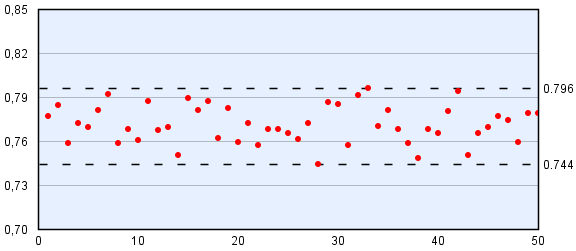
\includegraphics[scale=0.775]{images/MonteCarlo/1k.png}
  \caption{Result of the calculator with 1000 simulations \label{fig:mc1}}
\end{figure}

\begin{figure}[H]
  \center
    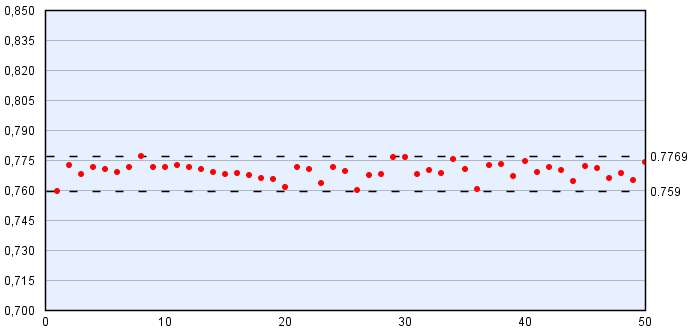
\includegraphics[scale=0.775]{images/MonteCarlo/10k.png}
  \caption{Result of the calculator with 10.000 simulations \label{fig:mc10}}
\end{figure}

\begin{figure}[H]
  \center
    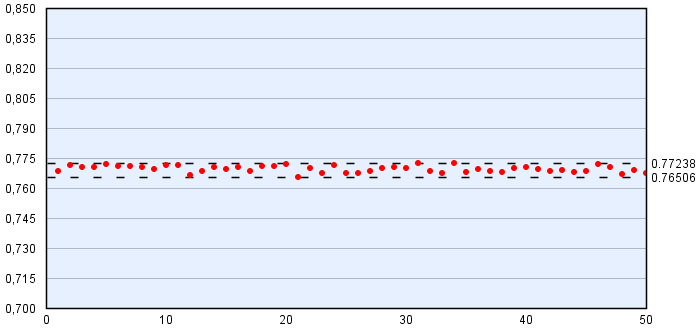
\includegraphics[scale=0.775]{images/MonteCarlo/50k.png}
  \caption{Result of the calculator with 50.000 simulations \label{fig:mc50}}
\end{figure}

\vspace{4mm}
\begin{table}[H]
  \center
  \begin{tabular}{ | l | l | l | l | }
    \hline
    simulations & range (\%) & max error (\%) & time (seconds) \\
    \hline                       
    1000 & 5,2 & 2,7 & 0,03 \\
    10.000 & 2,2 & 1,5 & 0,22\\
    50.000 & 0,9 & 0,7 & 0,82\\
  \hline  
  \end{tabular}
  \caption{Combined test results from running the calculator with different numbers of simulations. \label{tab:mc-total}}
\end{table}
\vspace{4mm}

\subsection{Discussion}
For our implementation of the calculator we use the Monte Carlo method. This method works well for our needs. The calculator can calculate the probability with an error percentage of less than one percent. This solution can be used for any poker state with up to ten players. We don't find it necessary to optimise the calculator any further, but it is currently only running a single thread. An obvious optimisation will be to make it multi-threaded.

Alternatively we could have created our own formula to calculate a rank, or used an existing one, for instance the Chen formula. By using this method we will get a less accurate result but it will be easier to calculate. We would also have to create a formula for each game state which would cause even more work. Since performance is not a problem for our calculator we chose to use the Monte Carlo method.

\subsection{Conclusion}
In this section we have answered the question:
\begin{quotation}
How can we predict the probability of ending up with the winning hand?
\end{quotation}

We have implemented a subsystem called the calculator that can estimate the probability of winning with a set of hole cards. The calculator uses the Monte Carlo method and it works for every poker state with up to ten players. We have found that 50.000 simulations is a good number of simulations for our calculator. 

We compare our results to caniwin, which is a website that has calculates the actual probabilities. The calculator has an error percentage of 0,7 percent and can perform the calculation in less than a second. The results of the calculator may vary up to one percent for any given poker state.